%%%%%%%%%%%%%%%%%%%%%%%%%%%%%%%%%%%%%%%%%
% Wenneker Article
% LaTeX Template
% Version 2.0 (28/2/17)
%
% This template was downloaded from:
% http://www.LaTeXTemplates.com
%
% Authors:
% Vel (vel@LaTeXTemplates.com)
% Frits Wenneker
%
% License:
% CC BY-NC-SA 3.0 (http://creativecommons.org/licenses/by-nc-sa/3.0/)
%
%%%%%%%%%%%%%%%%%%%%%%%%%%%%%%%%%%%%%%%%%

%----------------------------------------------------------------------------------------
%	PACKAGES AND OTHER DOCUMENT CONFIGURATIONS
%----------------------------------------------------------------------------------------

\documentclass[10pt, a4paper, twocolumn]{article} % 10pt font size (11 and 12 also possible), A4 paper (letterpaper for US letter) and two column layout (remove for one column)

%%%%%%%%%%%%%%%%%%%%%%%%%%%%%%%%%%%%%%%%%
% Wenneker Article
% Structure Specification File
% Version 1.0 (28/2/17)
%
% This file originates from:
% http://www.LaTeXTemplates.com
%
% Authors:
% Frits Wenneker
% Vel (vel@LaTeXTemplates.com)
%
% License:
% CC BY-NC-SA 3.0 (http://creativecommons.org/licenses/by-nc-sa/3.0/)
%
%%%%%%%%%%%%%%%%%%%%%%%%%%%%%%%%%%%%%%%%%

%----------------------------------------------------------------------------------------
%	PACKAGES AND OTHER DOCUMENT CONFIGURATIONS
%----------------------------------------------------------------------------------------

\usepackage[english]{babel} % English language hyphenation

\usepackage{microtype} % Better typography

\usepackage{amsmath,amsfonts,amsthm} % Math packages for equations

\usepackage[svgnames]{xcolor} % Enabling colors by their 'svgnames'

\usepackage[hang, small, labelfont=bf, up, textfont=it]{caption} % Custom captions under/above tables and figures

\usepackage{booktabs} % Horizontal rules in tables

\usepackage{lastpage} % Used to determine the number of pages in the document (for "Page X of Total")

\usepackage{graphicx} % Required for adding images

\usepackage{enumitem} % Required for customising lists
\setlist{noitemsep} % Remove spacing between bullet/numbered list elements

\usepackage{sectsty} % Enables custom section titles
\allsectionsfont{\usefont{OT1}{phv}{b}{n}} % Change the font of all section commands (Helvetica)

 \usepackage{setspace} \doublespacing 
\usepackage[switch]{lineno} 

% \usepackage{amsmath}
% \usepackage{breqn}
\usepackage{mathtools}

%----------------------------------------------------------------------------------------
%	MARGINS AND SPACING
%----------------------------------------------------------------------------------------

\usepackage{geometry} % Required for adjusting page dimensions

\geometry{
	top=1cm, % Top margin
	bottom=1.5cm, % Bottom margin
	left=2cm, % Left margin
	right=2cm, % Right margin
	includehead, % Include space for a header
	includefoot, % Include space for a footer
	%showframe, % Uncomment to show how the type block is set on the page
}

\setlength{\columnsep}{7mm} % Column separation width

%----------------------------------------------------------------------------------------
%	FONTS
%----------------------------------------------------------------------------------------

\usepackage[T1]{fontenc} % Output font encoding for international characters
\usepackage[utf8]{inputenc} % Required for inputting international characters

\usepackage{XCharter} % Use the XCharter font

%----------------------------------------------------------------------------------------
%	HEADERS AND FOOTERS
%----------------------------------------------------------------------------------------

\usepackage{fancyhdr} % Needed to define custom headers/footers
\pagestyle{fancy} % Enables the custom headers/footers

\renewcommand{\headrulewidth}{0.0pt} % No header rule
\renewcommand{\footrulewidth}{0.4pt} % Thin footer rule

\renewcommand{\sectionmark}[1]{\markboth{#1}{}} % Removes the section number from the header when \leftmark is used

%\nouppercase\leftmark % Add this to one of the lines below if you want a section title in the header/footer

% Headers
\lhead{} % Left header
\chead{\textit{\thetitle}} % Center header - currently printing the article title
\rhead{} % Right header

% Footers
\lfoot{} % Left footer
\cfoot{} % Center footer
\rfoot{\footnotesize Page \thepage\ of \pageref{LastPage}} % Right footer, "Page 1 of 2"

\fancypagestyle{firstpage}{ % Page style for the first page with the title
	\fancyhf{}
	\renewcommand{\footrulewidth}{0pt} % Suppress footer rule
}

%----------------------------------------------------------------------------------------
%	TITLE SECTION
%----------------------------------------------------------------------------------------

\newcommand{\authorstyle}[1]{{\large\usefont{OT1}{phv}{b}{n}\color{Black}#1}} % Authors style (Helvetica)

\newcommand{\institution}[1]{{\footnotesize\usefont{OT1}{phv}{m}{sl}\color{Black}#1}} % Institutions style (Helvetica)

\usepackage{titling} % Allows custom title configuration

\newcommand{\HorRule}{\color{Black}\rule{\linewidth}{1pt}} % Defines the gold horizontal rule around the title

\pretitle{
	\vspace{-30pt} % Move the entire title section up
	\HorRule\vspace{10pt} % Horizontal rule before the title
	\fontsize{32}{36}\usefont{OT1}{phv}{b}{n}\selectfont % Helvetica
	\color{Black} % Text colour for the title and author(s)
}

\posttitle{\par\vskip 15pt} % Whitespace under the title

\preauthor{} % Anything that will appear before \author is printed

\postauthor{ % Anything that will appear after \author is printed
	\vspace{10pt} % Space before the rule
	\par\HorRule % Horizontal rule after the title
	\vspace{20pt} % Space after the title section
}

%----------------------------------------------------------------------------------------
%	ABSTRACT
%----------------------------------------------------------------------------------------

\usepackage{lettrine} % Package to accentuate the first letter of the text (lettrine)
\usepackage{fix-cm}	% Fixes the height of the lettrine

\newcommand{\initial}[1]{ % Defines the command and style for the lettrine
	\lettrine[lines=3,findent=4pt,nindent=0pt]{% Lettrine takes up 3 lines, the text to the right of it is indented 4pt and further indenting of lines 2+ is stopped
		\color{DarkGoldenrod}% Lettrine colour
		{#1}% The letter
	}{}%
}

\usepackage{xstring} % Required for string manipulation

\newcommand{\lettrineabstract}[1]{
	\StrLeft{#1}{1}[\firstletter] % Capture the first letter of the abstract for the lettrine
	\initial{\firstletter}\textbf{\StrGobbleLeft{#1}{1}} % Print the abstract with the first letter as a lettrine and the rest in bold
}

%----------------------------------------------------------------------------------------
%	BIBLIOGRAPHY
%----------------------------------------------------------------------------------------
% \usepackage{natbib}
% \bibliographystyle{molecularEcology.bst}

\usepackage[backend=biber,style=apa,natbib=true]{biblatex} % Use the bibtex backend with the authoryear citation style (which resembles APA)

\addbibresource{tellis.bib} % The filename of the bibliography

\usepackage[autostyle=true]{csquotes} % Required to generate language-dependent quotes in the bibliography
 % Specifies the document structure and loads requires packages

%----------------------------------------------------------------------------------------
%	ARTICLE INFORMATION
%----------------------------------------------------------------------------------------

\title{Joint estimation of paternity, sibships and pollen dispersal in a snapdragon hybrid zone} % The article title

\author{
	\authorstyle{Thomas James Ellis\textsuperscript{1,2,3}, David Luke Field, \textsuperscript{1,3}, Nicholas H. Barton\textsuperscript{1}} % Authors
	\newline\newline % Space before institutions
	\textsuperscript{1}\institution{Institute of Science and Technology Austria, 2234 Klosterneuburg, Austria}\\ % Institution 1
	\textsuperscript{2}\institution{Gregor Mendel Institute of Molecular Plant Sciences, Dr.-Bohr-Gasse 3, 1030 Vienna, Austria}\\ % Institution 2
	\textsuperscript{3}\institution{Edith Cowen University, Perth, Australia} % Institution 3
}

% Example of a one line author/institution relationship
%\author{\newauthor{John Marston} \newinstitution{Universidad Nacional Autónoma de México, Mexico City, Mexico}}

\date{\today} % Add a date here if you would like one to appear underneath the title block, use \today for the current date, leave empty for no date

%----------------------------------------------------------------------------------------

\begin{document}

\maketitle % Print the title

\thispagestyle{firstpage} % Apply the page style for the first page (no headers and footers)
\linenumbers
%----------------------------------------------------------------------------------------
%	ABSTRACT
%----------------------------------------------------------------------------------------

% \lettrineabstract{}

\section{Abstract}
The distribution of pollen dispersal distances sets the scale for plant population dynamics.
A useful tool for inferring the distribution dispersal distances is to infer the distances between mates by paternity or parentage reconstruction.
This is most powerful when information about multiple properties or data types are inferred in a joint analysis.
We describe an approach to jointly infer paternity, sibling relationships and population parameters, with the example of the pollen dispersal kernel in a natural population of the snapdragon, \textit{Antirrhinum majus}.
The joint analysis gives a substantial increase in statistical power to identify fathers.
Pollen dispersal is leptokurtic, with half of mating events occurring within 30m, but with a long tail of mating events up to 2000m.
[Add a final sentence with about implications for the population. see Discussion].

%----------------------------------------------------------------------------------------
%	ARTICLE CONTENTS
%----------------------------------------------------------------------------------------

\section{Introduction}

Knowledge of the distribution of dispersal distances organisms or gametes travel during their lifetimes aids our understanding of natural populations because it sets the scale at which populations vary (\cite{cain2000long}).
For example, dispersal may enhance the response to selection by increasing genetic variance, may inhibit local adaptation via swamping by maladapted alleles, or alleviate inbreeding with nearby relatives (\cite{kremer2012long}).
Of particular interest is not the average distance travelled, but the shape of the dispersal distribution.
In plants, dispersal is often characterised by leptokurtic or 'fat-tailed' distributions, where dispersal is most likely to occur over short distances, but there is a long tail of long-range dispersal events (\cite{clark1998trees,austerlitz2004using,bullock2017synthesis}).
This leptokurtosis allows much more rapid dispersal than would be suggested by the average dispersal distance alone, with long-range migrants having a disproportionate effect on the spread of adaptive alleles (\cite{clark1998trees,cain2000long}).
We thus aim to accurately characterise the shape of dispersal distributions in natural populations.

A key tool for inferring dispersal is to infer the pedigree of relationships between individuals based on genetic information from parents and offspring, because this gives a direct estimate of the distances between mates (\cite{adams1992using, cain2000long, austerlitz2004using,pemberton2008wild}).
Pedigree inference is most successful when as much informative data as possible can be included in a joint analysis, such as from shared alleles between siblings, or phenotype information (\cite{neff2001bayesian, wang2007parentage}).
Dispersal is a clear example of this.
For example, one approach would be to infer a pedigree ignoring spatial information, then measure the distances between mates, assuming the pedigree to be correct.
This would overestimate average dispersal, because any candidates erroneously inferred to be parents will tend to be further apart than real parents.
Alternatively, one might first infer the distribution of dispersal distances using a non-genetic approach such as mark-recapture, then use this as a prior to inform pedigree inference.
This would underestimate dispersal, because such methods tend to miss dispersal events over longer distances.
By inferring pedigree relationships and dispersal jointly we can incorporate the information each has about the other and improve inference of both.

Several methods exist for the joint inference of parental relationships and other parameters.
Various approaches have been described to jointly infer sibling relationships with the parentage or paternity of those sibships (e.g. \cite{emery2001assignment, thomas2002sibship, jones2007estimating, wang2004sibship, anderson2016bayesian, huisman2017pedigree}).
Another approach is to include data about other biological parameters that might influence mating, such as relevant phenotypes or spatial information (\cite{neff2001bayesian, hadfield2006towards}).
This is especially appealling because it allows us to directly address biologically relevant relationships between traits of interest and mating patterns.
These approaches typically rely on an iterative algorithm such as simulated annealing or Monte-Carlo Markov chains (MCMC) to explore different pedigree structures.
This is time-consuming, especially for large samples, and there is no guarantee that the full space of plausible pedigree structures can be explored.
Moreover, we currently lack a framework for utilising all three sources of information - parentage, sibships and population parameters - in a single joint analysis.

We previously described a package Fractional Analysis of Paternity and Sibships (FAPS) to jointly infer of paternity and sibships (\cite{ellis2018efficient}), which we here extend to include inference of population parameters.
FAPS considers the probability of paternity of each offspring as a probability distribution over all candidate fathers simultaneously, and identifies and compares plausible sibling relationships.
In this way we can fully account for the uncertainty in paternal and sibling relationships in a few seconds, obviating the need to update pedigree relationships iteratively.
In this paper we describe how to include non-genetic information into the FAPS procedure, and use MCMC to update parameters for those data to jointly infer paternity, sibships and population parameters.
We then apply this to the inference of the pollen dispersal distribution in a hybrid-zone population of the snapdragon \textit{Antirrhinum majus}.

%------------------------------------------------

\section{Materials and Methods}

\subsection{\textit{A. majus} data}

\subsubsection{Study population}

\begin{figure*}
    \centering
	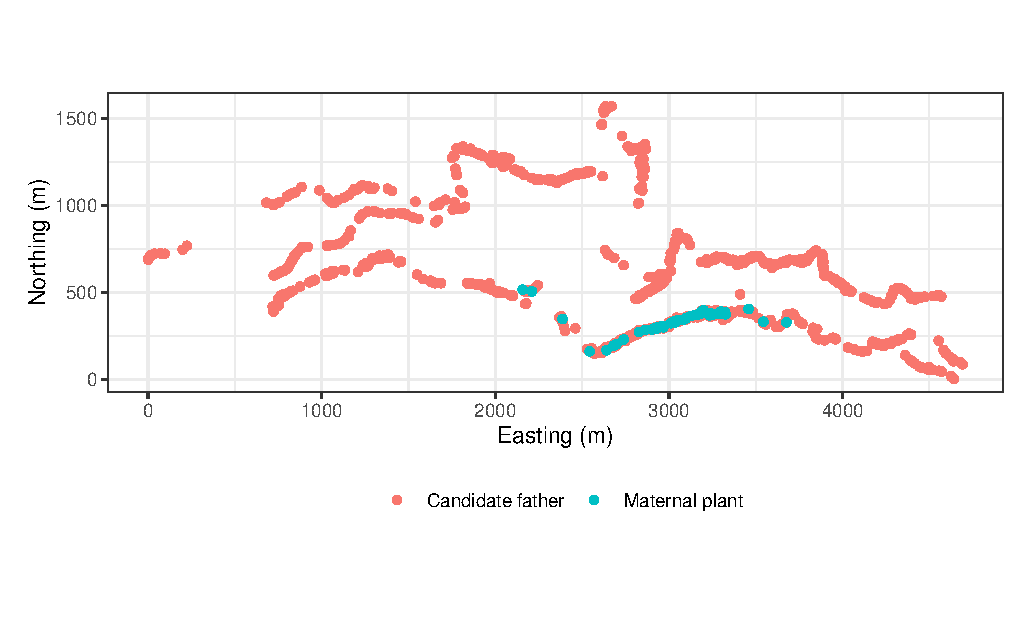
\includegraphics[]{map.eps} % Figure image
	\caption{
        Map of the hybrid zone.
        The map shows the distribution of maternal plants, inferred pollen donors and remaining plants along the lower (South) and upper (North) roads. Only pollen donors for families with one or more offspring are shown.}
	\label{fig:map} % Label for referencing with \ref{bear}
\end{figure*}

We examine a hybrid zone population of the snapdragon \textit{Antirrhinum majus} in the Spanish Pyrenees. Here, the yellow-flowered \textit{A. m. striatum} and the magenta-flowered \textit{A. m. pseudomajus} meet and hybridise to produce diverse recombinant phenotypes, including pink, white and orange flowers.
The population grows along two parallel roads running East-West close to Rib\"{e}s de Freser (figure figure \ref{fig:map}). The ’lower’ road is at 1150-1200m above sea level, whilst the ’upper’ road climbs 1250-1500m, and is 500-1000m north of the lower road. Hybrids are mostly confined to a 1km ’core’ hybrid zone, with \textit{A. m. striatum}- and \textit{A. m. pseudomajus}-like plants becoming dominant to the West and East respectively. We surveyed as many flowering plants as we could find in June and July of 2012 (n=2124), and collected information on flower number and location using a Trimble GeoXT datalogger. We collected two to three leaves for DNA extraction and dried these in silica gel (Fischer Scientific). \textit{A. majus} grows in disturbed habitats such as roadsides and railways; they are rare in the established forest and pasture between the two roads, on the north-facing slope to the South, and on the high mountain peak to the North of the two roads. It thus is likely that we sampled the majority of the plants that flowered during the study period, although we cannot exclude that some flowering may have occurred before or after this. 

Pollination is carried out exclusively by large bumblebees and carpenter bees who are large enough to open the flowers \cite{vargas2010occluded, andalo2019prevalence}. \textit{A. majus} has a gametophytic self-incompatibility system, and self-pollinated seeds are very rare. There are no detectable post-zygotic barriers between \textit{A. m. striatum} and \textit{A. m. pseudomajus} (\cite{andalo2010post}).

In August 2012 we collected a single, mature, wild-pollinated fruit from each of 60 mothers (figure \ref{fig:map}). In order to minimise disturbance to the population we only sampled from plants which had set a minimum of five mature fruits. These mothers were chosen to represent an even sample of pigmentation genotypes, spread as evenly as possible across the core of the hybrid zone where hybrids are most dense, resulting in 10 \textit{A. m. striatum}-like, 17 \textit{A. m. pseudomajus}-like, and 33 hybrid-phenotype mothers.

\subsubsection{Genotyping}

We grew seeds in 5cm plug trays filled with potting compost (Gramaflor) in a greenhouse under Sylvania GroLux lights on a 16-hour cycle. We sowed three seeds per plug for 50-70 plugs per maternal family and thinned seedlings to a single seedling per plug after cotelydons had appeared. We transferred approximately 1cm$^2$ of fresh tissue from 1419 seedlings to 96-well DNA-extraction plates (LGC Genomics, Berlin) and allowed tissue to dry using the sample bag and silica gel provided. For parental tissue from the hybrid zone we transferred approximately 1cm$^2$ tissue dried in the field to the same plates. DNA extractions of the plated tissue samples were carried out by LGC Genomics.

We genotyped tissue samples at 71 SNPs by KASPR sequencing (LGC Genomics). These SNPs are a subsample of a panel used for a wider survey of the hybrid zone (\cite{surendranadh2022effects}). The total SNP panel is a mixture of  diagnostic (showing a gradient in allele frequency across the hyrbid zone) and parentage (with as even a gradient in allele frequency as possible) SNPs. Previous work identified the per-locus genotyping error rate in these data to be approximately $10^4$ (coordinate on the pedigree paper for a citation). For parentage loci we chose only biallelic loci with a minor-allele frequency greater than 0.3 in each of inner four pools closest to the centre of the cline, selected to be at least 2cM apart. Diagnostic SNPs were either linked to pigmentation loci, or else showed sharp clines across the hybrid zone. We removed 474 offspring and four adults that had missing data at more than 7.5\% of the SNPs. We also pruned 7 SNPs that showed more than 10\% missing data, or less than 15\% heterozygosity. This left us with a set of 984 offspring from 60 maternal families, with between two and 29 offspring per maternal family (mean=16.4).

\subsection{Joint estimation of paternity, sibships and dispersal}

\subsubsection{Probability model}

We begin with observed SNP marker data \textbf{M} for mothers, offspring and candidate father, and a matrix \textbf{D} of Euclidean distances between mothers and all possible candidate fathers, as well as estimates $q$ of the proportion of candidate father sampled, and the per-locus genotyping error rate $\eta$. From this we wish to infer pedigree P describing sibling, paternal and (known) maternal relationships, and vector $\theta$ of dispersal parameters. The full probability model is then

\begin{equation}
\label{eqn:probability_model}
\begin{split}
\Pr( P, \theta | \textbf{M}, \textbf{D}, q, \eta) \propto \Pr(\textbf{M} | P, \textbf{D}, q,\theta, \eta)
\Pr(\textbf{D} | \theta, P) \\
\Pr(\theta) \Pr(P) \Pr(\eta)
\end{split}
\end{equation}

In the following sections we outline how to extend our existing method for inferring sibships and paternity to include data from non-genetic covariates, a model for pollen dispersal, suitable hyperprior distributions for dispersal parameters, and a procedure to infer the posterior distribution of the parameters of interest.

\subsubsection{Allowing for covariates in paternity inference}

We have previously described a Python package FAPS which performs joint analysis of paternity and sibship relationships for sibling arrays based on SNP data, and allows for integrating out uncertainty in relationships (\cite{ellis2018efficient}). Here we extended the software to allow for additional non-genetic information to be included.

FAPS begins with marker data for one or more maternal families composed of a mixture of half- and full-siblings, the known mother of each family, and an array of candidate fathers.
\cite{ellis2018efficient} described a method to infer sibling and paternity relationships in those individuals; we refer the reader to that paper for the full details, but review the most important aspects here.
FAPS uses marker data \textbf{M} to build matrix \textbf{G} of probabilities of paternity based on Mendelian transition probabilities for each maternal family. \textbf{G} has a row of each offspring and a column for each candidate father, where element $g_{ij}$ is the probability that candidate \textit{j} is the father of offspring \textit{i} given marker data, an estimate of genotyping error rate $\eta$, and an estimate of the proportion of missing candidate fathers $q$. Rows in \textbf{G} sum to one, and describe a multinomial distribution of probabilities of paternity over all candidate fathers. The final column of \textbf{G} is the probability that the father of each offspring was missing from the sample of candidates, based on the probability of observing offspring alleles from population allele frequencies, and an estimate of the proportion of possible pollen donors in the population that had been sampled. FAPS then builds a similarity matrix whose \textit{ih}\textsuperscript{th} element is the likelihood 

\begin{equation}\label{eqn:faps_similarity_matrix}
\Sigma_j^F g_{ij}g_{hj}
\end{equation}
that the \textit{i}\textsuperscript{th} and \textit{j}\textsuperscript{th} offspring are full siblings by summing over the probabilities that they share any one of the $F$ fathers. The similarity matrix is used to perform hierarchical clustering to identify plausible ways to partition offspring into families of possible full sibships, and the likelihood of each partition structure is estimated by Monte-Carlo simulation. The likelihood that candidate father \textit{j} is the father of putative full sibship \textit{k} is then

\begin{equation}\label{eqn:faps_lik_sibship}
\Pi_i^n g_{ij}
\end{equation}
for all \textit{n} offspring in \textit{k}. FAPS returns a vector of probabilities (which sum to one) that each candidate is the father of sibship \textit{k}, or that the true father was not sampled. This is done for each plausible partition structure. This gives a distribution of possible partition structures and their likelihoods, and a distribution of paternity probabilities for each putative family within each partition structure.

We can incorporate non-genetic information about paternity using a suitable function relating those data into probabilities of paternity.
In principle this can be done for any kind of data for which there is a suitable function relating the observed data for a set of candidate fathers to a probability of having mating with each mother, given a set of parameter values for that function. The goal is to find parameter values that best explain the data. For example, a standardised continuous phenotype $z$ could be modelled with the logistic function $1/1+\exp{\beta z}$, where $\beta$ describes the relationship between $z$ and male fertility. A categorical phenotype can be modelled as a multinomial vector of probabilities that sum to one. In this study we use matrix \textbf{D} of Euclidean distances between mothers and candidate fathers as a covariate, and model the probability $\Pr(d_{mj}|\theta)$ of a mating event occurring between mother \textit{m} and candidate \textit{j} who are distance $d_{mj}$ apart, based on a suitable model of pollen dispersal (see below). It is then straightforward to incorporate this into the procedure outlined above by modifying eqn. \ref{eqn:faps_similarity_matrix} to

\begin{equation}\label{eqn:pairwise_with_covariates}
\Sigma_j^F \Pr(d_{mj} | \theta)g_{ij}g_{hj}
\end{equation}

and eqn. \ref{eqn:faps_lik_sibship} to

\begin{equation}
\label{sibship_with_covariates}
\Pr(d_{mj} | \theta)\Pi_i^n g_{ij}
\end{equation}

Eqn. \ref{sibship_with_covariates} can then be used to estimate the likelihood of the partition structure by Monte-Carlo simulation, as previously described by \cite{ellis2018efficient}.
For a given set of dispersal parameters in $\theta$ the likelihood of the whole maternal family is then the sum of likelihoods for each possible partition. When there are multiple maternal families, the likelihood of the whole dataset given $\theta$ is the product of those likelihoods over each maternal family. When we update $\theta$, this likelihood will change, giving us a way to compare likelihoods of different dispersal parameter values and identify those most consistent with the data.

A special case arises when it is known that offspring are unrelated, or that sibship structure is otherwise known. In this case the likelihood of the data can be calculated by summing the likelihoods of paternity for each candidate father on the $k^{th}$ full-sibship, and multiplying over all $K$ full sibships:

\begin{equation}
\label{lik_if_no_structure}
\Pi_k^K\Sigma_j^F\Pr(d_{mj} | \theta)\Pi_i^n g_{ij}
\end{equation}

This obviates the need for likelihood estimation by Monte-Carlo simulation.

\subsubsection{Pollen dispersal distribution}

A useful function for describing plant dispersal distributions is the generalised normal distribution (\cite{clark1998trees,Nadarajah2005,kremer2012long}). This is a generalisation of the exponential family of probability distributions and includes the exponential and standard normal distributions as special cases, but allows for fat and thin tails. It is commonly used to model plant dispersal distributions because these are often found to show clear kurtotis (e.g. \cite{austerlitz2004using, robledo2005patterns, klein2008pollen, burczyk2019patterns, field2011importance, ottewell2012pollen}). The generalised normal distribution describes the probability of observing dispersal distance \textit{d} given scale parameter $a$ and shape parameter $b$:

\begin{equation}
\Pr(d|a,b) =K e^{  (-\frac{d}{a} )^b }
\label{eqn:GND}
\end{equation}

where K is normalising constant $b/[2a\Gamma(1/b)]$ and $\Gamma$ is Euler's gamma function. The function takes the forms of the standard exponential and normal distributions when $b=1$ and $b=2$ respectively. Values of $b<1$ reflect leptokurtic distributions with tails that decay more slowly than would be expected under the exponential distribution. Using $\theta={a,b}$, this provides a convenient function for calculating $\Pr(d_{mj} | \theta)$ because it allows for a long tail of long-distance migrants.

However, although leptokurtosis of an inferred dispersal distribution may be caused by genuine distant mating events, the tail of the distribution may also be inflated by incomplete sampling of true fathers. Because rows of \textbf{G} must sum to one the absence of the true father increases the probability of paternity of unrelated candidates, some of whom may have high probabilities of paternity of one or more offspring just by chance. Whereas true fathers are expected to be (on average) close to the mother, other candidates should be drawn at random from the population, since the marker set is designed to show as little spatial structure as possible. This will inflate the apparent kurtosis in the data and underestimate $b$. To accommodate this we modify the model above to model dispersal as a mixture of a generalised-normal and a uniform distribution:

\begin{equation}\label{eqn:mixture_model}
\Pr(d_{mj} | a,b,\lambda) = \lambda \Pr(d_{mj}|a,b) + \frac{1-\lambda}{F}
\end{equation}
where F is the number of candidate fathers and $\lambda$ is a mixture parameter determining the proportion of the probability mass due to ’real’ dispersal. The uniform part of this mixture allows for signal coming from incorrect candidates without requiring the 'true' dispersal kernel to be unnecessarily leptokurtotic. Conveniently, also provides an estimate of the false positive rate if we had run paternity analysis using genetic data alone.

It is common to also report the mean dispersal distance as the second moment of this distribution as
\begin{equation}
\label{eqn:sd_GND}    
\sqrt{ \frac{ a^2 \Gamma(3/b) }{ \Gamma(1/b) } }
\end{equation}
We prefer to focus on median dispersal distances because this is more intuitive for highly skewed distributions, and also to estimate this on realised inter-mate distances rather than on parameters alone (see "Inference of mating patterns"). We nevertheless report this and how it relates to the effect of $\lambda$ on results.

\subsubsection{Priors for dispersal parameters}

We require prior distributions for dispersal parameters $a$, $b$ and $\lambda$.

We used a log-normal prior for $b$ ($exp{b} \sim N(\mu=0, \sigma = 0.5)$.
This model allows for a range of shape values reflecting leptokurtosis to Gaussian dispersal, but is skeptical about very strong over- or under-dispersion in the dispersal distribution because prior probabilties approach zero as $b$ approaches 0 or 3 (figure S1).
We used a Gamma prior for $a$ because this describes positive continuous values, and because it is conjugate with the variance parameter of a Gaussian distribution.
Because the effect of $a$ depends on $b$ and has no intuitive biological interpretation itself, we used prior simulations to choose a suitable parameterisation for $a$. We first simulated 10000 pairs of values for $a$ and $b$ from Gamma and log-normal distributions respectively. We then used each pair of simulated values to parameterise a generalised normal distribution, and simulated 1000 dispersal distances from that distribution, and visually examined the distribution for biological plausibility. We chose a Gamma distribution with shape=6 and scale=50, because this gave dispersal distributions with most dispersal occurring within 500m, but allowing for rare long-range dispersal events (figure S1).

For $\lambda$, we use a beta distribution with parameters Beta(1.1, 1.1).
This distribution approaches zero when $\lambda$ is close to zero or one, but is fairly flat in between.
This implies that we do not expect that all the weight should be on either the generalised-normal or the uniform components of the mixture distribution in eqn. \ref{eqn:mixture_model}, but that we do not have strong prior beliefs about values between that.
To examine the effect of modelling dispersal as a mixture model at all, we also repeated the MCMC with with $\lambda$ to set to one.

\subsubsection{Inference via MCMC}

We used the Metropolis-Hastings Markov-chain Monte Carlo algorithm to infer the posterior distribution of dispersal parameters $a$,$b$ and $\lambda$.
Ideally we would also like to estimate the posterior distribution of the proportion of missing fathers $q$, but we found this to be unstable.
Moreover, we demonstrate by simulation that varying this parameter has negligible effect on biological conclusion (see below).
We therefore used a fixed value of $q=0.5$, which is tantamount to a flat prior on sampling effort. 

We ran four independent chains beginning from distant areas of the parameter space.
At each iteration, we perturbed the value of each parameter by a factor drawn from a normal distribution with a fixed standard deviation for each parameter ($\sigma= 2$ for $a$; $\sigma= 0.05$ for $b$; $\sigma= 0.025$ for $\lambda$).
We ran each chain for 40000 iterations and subsequently removed the first 500 iterations of each as burn-in.
After checking chain convergence (figures S2-S4) we thinned subsequent iterations to retain 250 posterior draws from each chain for further analyses, for a total of 1000 posterior draws.

\subsubsection{Inference of mating events}

We aimed to create a list of possible mating events between mothers and candidate fathers consistent with the data to identify a set of independent pollen dispersal events.
For each partition structure, FAPS identifies valid set of distinct fathers for each full sibship, and estimates a likelihood for each father-sibship configuration.
Each set of fathers reflects a hypothetical set of mating events, and the probability that a single father mated with the maternal plant is the sum of probabilities for each partition structure in which he sires at least one offspring.
This gives a list of mating events, with a posterior probability that each occurred, including an entry for offspring whose father was missing.
The posterior estimate of offspring number is the number of offspring for each father in each father-sibship configuration weighted by the probability of the mating event.
Note that the number and size of sibships are not necessarily integers because estimates are weighted averages.
In particular, hypothetical families can have posterior sizes less than one if the nominal number of offspring is one, but the posterior probability for the family is less than one.

The total number of mating events is the sum of probabilities for all mating events with sampled fathers.
Likewise, an estimate of the number of missing fathers is the sum of probabilities for all mating events for unsampled fathers.
However, FAPS does not distinguish paternal families within groups of offspring of an unsampled father, so this value is a lower bound on the number of unsampled fathers.

For 1000 iterations of the MCMC output we inferred mating events in this way, based on genetic information and probabilities of dispersal from the scale and shape values for that iteration in sibship clustering (eqn. \ref{eqn:pairwise_with_covariates} and \ref{eqn:faps_lik_sibship}). This gives 1000 sets of mating events for each iteration of the MCMC output.

Finally, we estimated the relationship between the number of offspring in a maternal array and the number of paternal families therein.
We first averaged paternal family size for each mother-father pair over iterations of the MCMC, then fitted a Poisson generalised linear model (GLM) of paternal family size on maternal family size (\cite{McCullagh1989}).

\subsection{Power analysis}

We used simulations to determine the statistical power of the dataset and method to identify true fathers.
We simulated mating events based on pollen dispersal from 200 draws from the posterior distributions of shape and scale parameters.
For each iteration in the chain we simulated mating events between each true mother and one or more sires drawn from the pool of genotyped adult plants.
We drew sires based on the probability of mating with a mother given dispersal parameters for that iteration.
For each mother, we simulated as many mating events of the same size as were inferred in that mother in the observed data.
We ignored mating events with posterior probabilities less than 0.9.
We simulated offspring genotypes based on Mendelian segregation and added genotyping errors to adults and offspring genotypes with the observed genotype error rate of $10^{-4}$ per locus per individual.
In this way simulated data reflects the structure of the empirical dataset.

We also investigated the relationship between the true proportion of missing fathers and prior assumptions about sampling effort.
To do this we randomly removed 10\%, 30\% or 50\% of the true fathers for each simulated dataset.
We then used FAPS to infer mating events for each dataset using prior probabilties of the proportion of missing fathers of 10\%, 20\%, 30\%, 40\% and 50\% and counted how often we were able to recover correct paternal families, the number of incorrect paternal families and the number of offspring assigned to missing fathers.
This simulates the effect of incomplete sampling, as well as of over- and under-estimating incomplete sampling in subsequent analysis.

\subsection{Asymmetric dispersal}

To test for potential bias in the direction of pollen dispersal we calculated the mean difference in East-West position between mothers and fathers.
We compared the average asymmetry in direction for observed mating events to simulated mating events as described above.
Because all but one observed pollen donor turned out to be on the lower road we restricted this analysis to simulated pollen donors on the lower road as well.

\section{Results}

\subsection{True sibships can be identified with high confidence}

\begin{figure*}
    \centering
    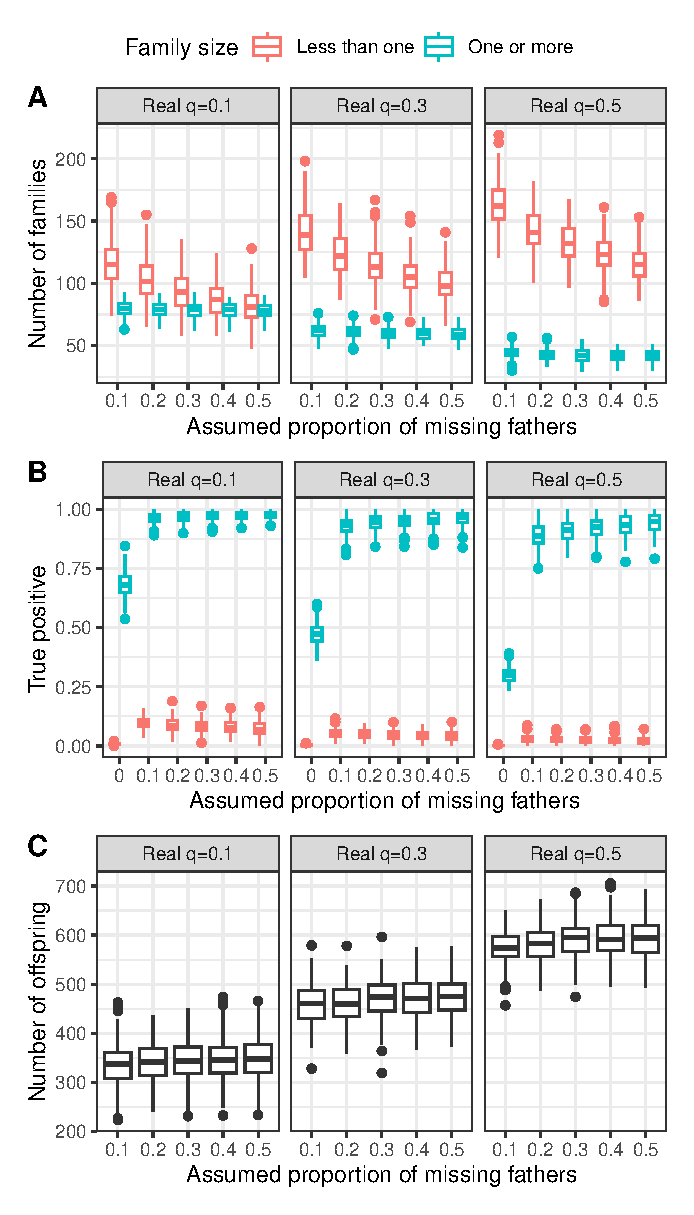
\includegraphics{simulations.eps}
    \caption{
        Simulation results.
        Panels show the true proportion of missing father; \textit{x}-axes show the assumed proportion used to infer families.
        (A) Number of paternal families identified with weighted-mean offspring number averaged over plausible sibships greater or less than one.
        (B) Probability that paternal families identified by FAPS are real.
        (C) Number of offspring inferred to have an unsampled father.
    }
    \label{fig:simulations}
\end{figure*}

We found that paternal families inferred from simulated data could be divided into those with family sizes of one or more, and a second group with weighted-mean family sizes less than one (figure \ref{fig:simulations}A).
The latter category occurs when one offspring in a full-sib family is compatible with a candidate father who is not the true father, leading to a paternal family of size one with posterior probability less than one.
Consistent with this, families with one or more offspring overwhelmingly reflect true mating events, whereas those with less than one offspring were overwhelmingly incorrect (figure \ref{fig:simulations}B).
This indicates that we can reliably identify true mating events by discarding paternal families with weighted-mean family sizes less than one.

We found surprisingly little effect of prior beliefs about the proportion of missing fathers on the accuracy of paternity inference.
Focussing on robust paternal families with one or more offspring, the number of families detected decreased as the true number of missing fathers increased, as one would expect (figure \ref{fig:simulations}A).
However, there was negligible relationship between the number of these families found and the prior expectation about the proportion of missing fathers, even when this prior substantially over- or under-estimated the true value.
We did find a slight increase in the probability that these inferred mating events were correct with higher input values of $q$ (figure \ref{fig:simulations}B), presumably because increasing the prior probability that a father is unsampled decreases the probability of paternity for candidates who are not true fathers.
Likewise, the number of offspring assigned to missing fathers increased with the true proportion of missing fathers, but there was no effect of changing the value of proportion of missing fathers used in the analysis (figure \ref{fig:simulations}C).
These results demonstrate that the prior expectations about the proportion of missing fathers has very little effect on downstream analyses.

\subsection{Number and size of full-sibling families}

We identified an average of 160.6 full-sibling families for which a father could be positively identified across MCMC samples (96\% credible intervals (CI): 156, 163).
Consistent with simulation results, 18.6 families had posterior-mean family sizes less than one (96\% CIs: 14, 121; figures S2, S3).
These families typically had posterior probabilities less than one and showed substantial uncertainty across MCMC iterations, indicating that they were detected only for a subset of possible sibship configurations (figure S2).
In contrast, the remaining 142.0 families had posterior probabilities greater than 0.99 and were found across MCMC iterations, indicating that these families are genuine (figure S2).
These paternal families likely reflect robust independent mating events that can be used to infer a dispersal kernel.

Full-sibship sizes ranged from one to 15 (figure S3).
The GLM of the number of full sibships on maternal-family size revealed that log number of sibships increased by 0.066 ($\pm$0.015) for every additional offspring included in the maternal family (intercept = -0.173 $\pm$ 0.307; figure S4). This corresponds to detecting a new family for approximately every 3 or 4 offspring genotyped, on average.

For all sixty mothers we found a mating event with non-zero probability for which the father one or more offspring was not sampled.
These families include an average of 590.2 offspring (CIs: 588.3, 592.3).
This corresponds to around 60\% of the offspring, and a minimum of 28.1\% (CIs 27.8, 28.3) of the total sample of pollen donors.
This discrepancy arises because an unsampled fathers may sire more than one offspring, and this analysis does allow us to distinguish multiple paternal families among offspring whose father was not sampled.

\subsection{Pollen dispersal is leptokurtic and asymmetric}

\begin{figure*}
    \centering
    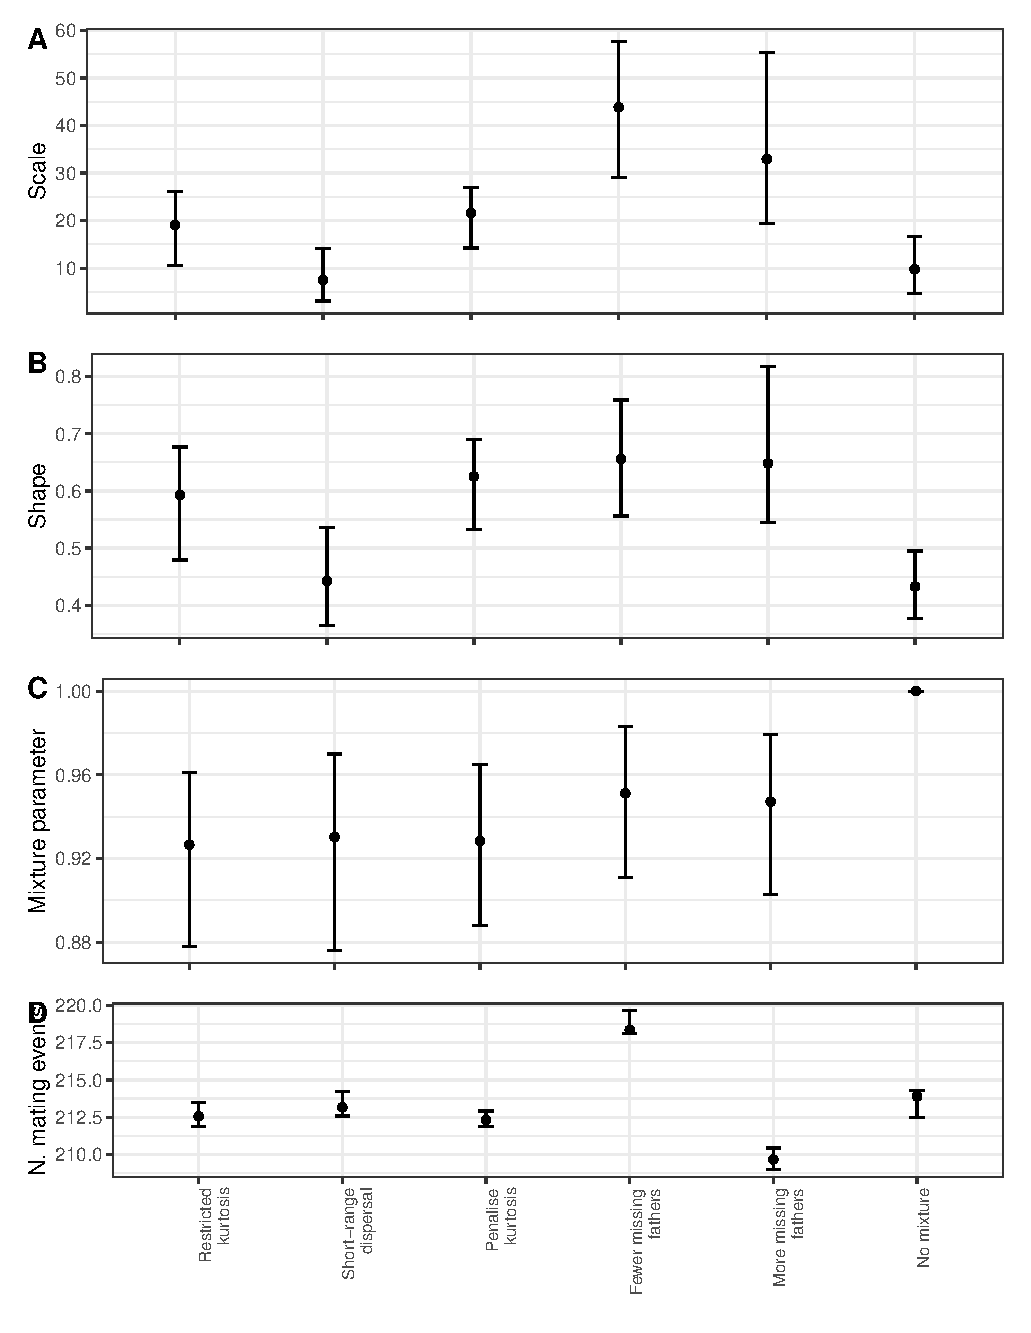
\includegraphics{posterior_distributions.eps}
    \caption{
        Posterior densities for the scale, shape, and mixture parameters of the dispersal kernel.
        Histograms show stacked densities for each of four independent chains.
    }
    \label{fig:posterior_summaries}
\end{figure*}

\begin{figure*}
    \centering
    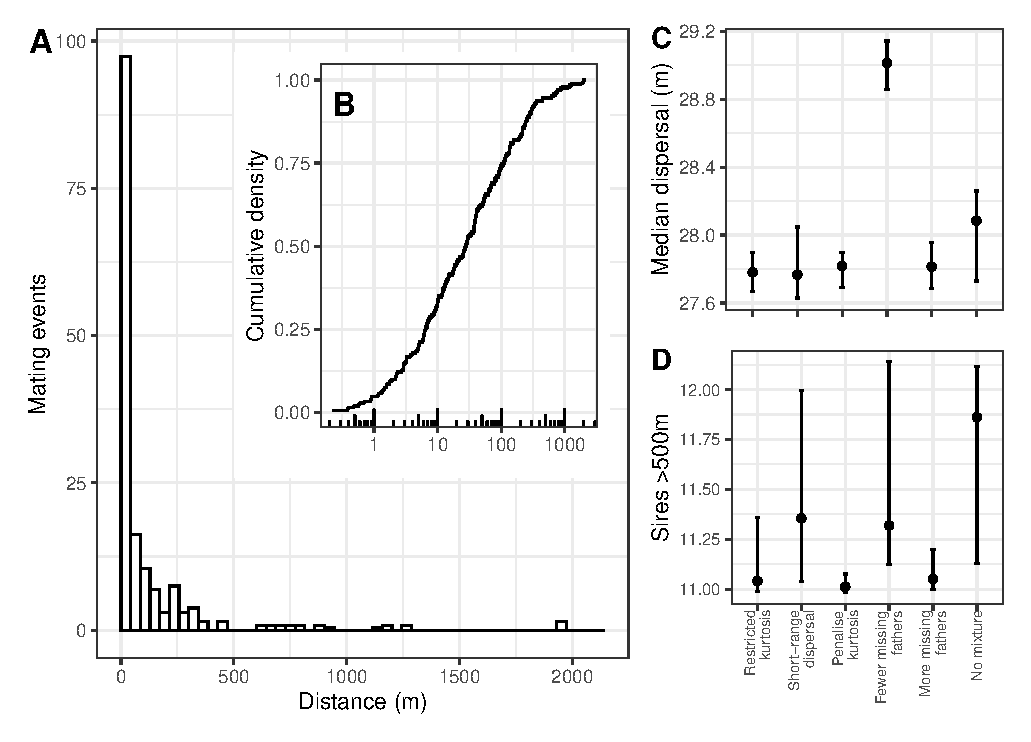
\includegraphics{dispersal.eps}
    \caption{
        Distribution of pollen-dispersal distances.
        (A) Histogram and (B) cumulative distribution of distances for dispersal events for paternal families with one or more offspring.
        Note the log10 scale of the x-axis in B.
        Mating events are weight weighted by their posterior probability.
        The histogram is summed over iterations of the MCMC.
        Separate cumulative curves are shown for 1000 MCMC iterations separately.
    }
    \label{fig:dispersal}
\end{figure*}

Across prior dispersal scenarios, independent MCMC chains converged on the stationary and were generally well mixed (figures \ref{fig:posterior_summaries}, S4).
The posterior distribution for the disperal shape parameter was consistently less than one, with a posterior mean of 0.56 (96\% CIs: 0.46, 0.70), indicating a leptokurtic dispersal kernel (figure \ref{fig:posterior_summaries}B).
Consistent with this, the distribution of pollen dispersal distances shows a peak close to zero and a long tail of long-distance dispersal events up to 747m (figure \ref{fig:dispersal}A).
Mean and median dispersal distances were 78.0 and 26.7 metres respectively.
With one exception, all mating occured between plants on the lower road.

Pollen donors were on 26\% more likely to be to the East of the maternal plants they mated with.
Simulated pollen donors were 5.1\% more likely to be to the East of their mates, indicating that this is at least partially due to increased density of plants to the East of the sample of maternal plants.
Nevertheless the average position of observed pollen donors was 36.7 metres further to the East than their mates, which is further than in 98.0\% of simulated datasets (mean distance = 12.8 metres; 96\% CIs: -5.93, 32.7).
This indicates that there is a bias in pollen flow favouring Westward dispersal.

\subsection{Mixture parameter reduces bias in dispersal shape}

The posterior distribtion the mixture parameter $\lambda$ was centred around 0.93 (96\% CIs: 0.88, 0.96; figure \ref{fig:posterior_summaries}C).
The precise interpretation of this number is somewhat obscure, but the fact that this number is close to, but not equal to zero indicates that at least small proportion of sires are missing, and that other non-sires located far from the mother have high probabilities of paternity by chance.
If ignored, this signal would inflate apparent leptokurtosis in the dataset.
Consistent with this, when we constrain $\lambda$ to be fixed at one the posterior distributions for the scale and shape parameters are shifted downwards compared to the analysis where $lambda$ is allowed to vary (posterior means drop from 17.5 to 17.1 and from 5.6 to 4.9 respectively).
This would indicate a more leptokurtic pollen dispersal kernel (figure \ref{fig:posterior_summaries}A, \ref{fig:posterior_summaries}B).
This in turn implies a substantial increase in mean dispersal distance (estimated as the second moment of the generalised normal distribition from eqn. \ref{eqn:sd_GND}) from 114 to 193 metres (figure S7).
Fortunately, there was no difference in mean or median dispersal distance based on realised mating events.
In this instance then, including a mixture component in the dispersal kernel reduces the bias caused by missing fathers in dispersal shape and apparent mean dispersal distance when this is inferred from the shape of the dispersal distribution.
However, this does not have a large enough impact on realised dispersal distances in these data to greatly affect biological conclusions.

\section{Discussion}

We have described a framework to jointly infer paternity, sibling relationships and population parameters. Simulations showed that using all three sources of information leads to a substantial increase in statistical power to identify fathers correctly compared to using paternity, or paternity and sibship information alone. Applying this to a natural populations of snapdragons, we find strong evidence for a leptokurtic pollen-dispersal kernel, which is robust to prior assumptions about dispersal and sampling effort.

\subsection{Performance of the method}

Our results showed that when a father is present we ought to be able to identify him with high probability using this marker set (figure \ref{fig:simulations}).
Where there is uncertainty about whether a specific mating event occurred, this is for sibships with fewer than one offspring (figure S5).
This is because we focus on whether a candidate mated with a mother at all, integrating out the uncertainty in sibship structure.
This idea is not necessarily intuitive, so to illustrate this, imagine three offspring (A, B and C) with two candidate fathers (X and Y).
There are two plausible paternal-sibships configurations,: (1) X is the father of A, B and C, with probability 0.6, or (2) X is the father of A and B, while Y is the father of C with probability 0.4.
The probability that X mated with the mother is 0.6+0.4=1, but the probability that Y mated with the mother is 0.4.
Weighted mean offspring numbers are (3*0.6)+(2*0.4)=2.4 for X and 1*0.5=0.5 for Y.
Thus the uncertainty in the paternity of offspring C causes uncertainty about the existence of the mating event with candidate Y.
We cannot say for certain that none of the sibships inferred to have fewer than two individuals are correct or not. 
However, by specifying the range of plausible sibship structures and the support for each, we can quantify this uncertainty and factor it out of our downstream results.
In contrast, in previous simulations to test the performance of FAPS we focussed on the most likely partition structure to simplify results, and found that the main source of error was individuals from a larger sibship group being falsely assigned to a singleton sibship (\cite{ellis2018efficient}).
This demonstrates the value of accounting for uncertainty in pedigree structure as well as possible.

We estimated that at least 21\% of fathers are likely to be missing from the population sample.
This number is certainly an underestimate of the true value, but there is reason to think that the true value is not substantially higher.
First, changing the prior on the proportion of missing fathers had only a minor effect on this estimate.
Second, we found that increasing the prior to 0.42 the MCMC behaved poorly, suggesting that this is a poor fit to the data.
Third, this estimate is similar to estimates by [other stuff Dave and Nick have done - please can you add something?], and we expect the estimate here to be lower because all the fathers have to have flowered in 2012.
The proportion of missing fathers is important, because missing fathers will cause false paternity to unrelated fathers, biasing dispersal estimates.

We modelled dispersal as a mixture distribution with a term allowing for false positive fathers to try and reduce the bias in estimates of dispersal.
The mixture distribution reduces the bias in the estimated shape parameter and the second moment of the generalised normal distribution, often interpreted as mean dispersal distance.
We note that this bias will exist as long as knowledge of paternity is less than perfect, and as such the mixture model reduces, but probably does not completely eliminate, this bias. 
Fortunately our biological conclusions are not affected, because we focus on the distribution of realised mating events, which are affected in only a minor way in real terms (figure \ref{fig:dispersal}C, \ref{fig:dispersal}D).
However, caution is warranted in the interpretation of the raw parameter values for shape and mean dispersal from the generalised normal distribution (figure S7).
It is possible that the effect was stronger here than would be the case in other published studies because our sample of candidate fathers is large, and the spatial extend is much larger (two orders of magnitude) than median dispersal distance.
In contrast, other studies have focussed on wind-pollinated trees, where pollen can travel much further, and had smaller numbers of candidates (e.g. \cite{adams1992using, austerlitz2004using, klein2008pollen}).
This demonstrates the utility of using inferred dispersal parameters to inform inference of real mating events, rather than focussing on the parameters themselves.

\subsection{Comparison with dispersal in other systems}

The results are similar to those found by Field et al. (in prep.) in the same population.
That study used a much large sample of individuals from multiple years and sought to infer the full multi-year pedigree.
The distribution of inter-mate distances was also fat-tailed, with a somewhat higher median distance of [number]m.
This difference in dispersal distances is to be expected.
First, the search space for identifying parents is much larger, because both parents need to be identified rather than just the father, and because parents may have been sampled over multiple years.
Second, although the pedigree is based on more genetic markers, there was no explicit model of dispersal.
Third, the present study considers only a single year; it is likely that the shape and location of the dispersal kernel would vary between seasons.
Despite these differences, the close concordance in results between these two studies indicates that the results are largely replicable.

The finding of leptokurtic dispersal is also consistent with other studies of plant dispersal
A meta-analysis of seed dispersal kernels found that the generalised normal distribution was a good fit for 86\% of datasets examined, and in 87\% of those cases the distribution was leptokurtic.
Fewer studies have been performed on pollen dispersal, but these commonly reported leptokurtic shapes as well (e.g. \cite{adams1992using, austerlitz2004using, robledo2005patterns, klein2008pollen, burczyk2019patterns}, but see \cite{field2011importance} or \cite{ottewell2012pollen} for counter examples).
All of these studies examined tree populations; to our knowledge ours is the first to estimate dispersal in a non-tree species.

\textit{A. majus} is specialised on large bee species for pollination, with the majority of pollination visits performed by the bumblebee species \textit{Bombus hortorum} and \textit{B. terrestris} (\cite{vargas2010occluded, andalo2019prevalence}.
The observation half of pollination events happen within 30m is consistent with bumblebees foraging on local patches of rewarding flowers close to a nest, but it is more surprising that a large fraction of pollination events take place over the scale of kilometres.
However, estimates of \textit{Bombus} foraging distances range from hundreds of metres (\cite{osborne1999landscape, wolf2008foraging}) to kilometres (\cite{osborne2008bumblebee, hagen2011space}).
In particular, queen bumblebees have been reported to disperse over many kilometres (\cite{lepais2010estimation}), and are frequent visitors to Antirrhinum because of the high nectar reward on offer.
Queen bumblebees appear very early in the season, so one explanation for some of the missing fathers from our dataset is that pollination occurred before the sample period.

\subsection{Implications for the hybrid-zone population}

The shape of the dispersal kernel implies that most mating occurs within tens of metres, but that there is a long tail of mating events between individuals at up to 2 km. This result suggests that any natural selection acting through male reproductive components (pollen dispersal) is occurring at small spatial scales. If pollinators discriminate between different flower-colour phenotypes in the hybrid zone, this sets an important geographic scale of selection for empirical tests on pollinator-mediated selection. For example, within 20m in the core of the hybrid zone, pollinators would encounter a full range of colour phenotypes that would provide scope for colour discrimination and differential visitation to influence male and female fitness. In this paper we have not attempted to estimate selection via flower colour because the number of mothers for each flower colour is small, meaning that we likely have little statistical power. However, in ongoing work we are investigating variation in fitness in a much larger panel of offspring arrays, which will allow us to address such question with much greater accuracy.

Paragraph about impact on small scale.
For example, link to inbreeding paper.
Link to self-incompatibility system?

Paragraph about impact of long-range dispersal events
How much pollen could cross the HZ?
How does that affect clines?
We didn't find evidence of asymmetry that might indicate a barrier to introgression, but this dataset focussed on the core, so it isn't a great sampling design to test that.

\section{Acknowledgements}

We thank a large number of field volunteers for maintaining the population sampling, and Tom White for assistance with seed collection. We thank Sylvia Rebel for plating tissue for DNA extraction.
We thank Barton group members for critical comments on this manuscript, even if they do not yet know it at the time of writing.

\section{Data availability}

Data and code to recreate the analyses will go on Zenodo, but for now they are available at \url{https://github.com/ellisztamas/amajus_dispersal_ms}.

%----------------------------------------------------------------------------------------
%	BIBLIOGRAPHY
%----------------------------------------------------------------------------------------

\printbibliography[title={Bibliography}] % Print the bibliography, section title in curly brackets

%----------------------------------------------------------------------------------------

\end{document}
